\documentclass[11pt]{article}\usepackage[]{graphicx}\usepackage[]{color}
%% maxwidth is the original width if it is less than linewidth
%% otherwise use linewidth (to make sure the graphics do not exceed the margin)
\makeatletter
\def\maxwidth{ %
  \ifdim\Gin@nat@width>\linewidth
    \linewidth
  \else
    \Gin@nat@width
  \fi
}
\makeatother

\definecolor{fgcolor}{rgb}{0.345, 0.345, 0.345}
\newcommand{\hlnum}[1]{\textcolor[rgb]{0.686,0.059,0.569}{#1}}%
\newcommand{\hlstr}[1]{\textcolor[rgb]{0.192,0.494,0.8}{#1}}%
\newcommand{\hlcom}[1]{\textcolor[rgb]{0.678,0.584,0.686}{\textit{#1}}}%
\newcommand{\hlopt}[1]{\textcolor[rgb]{0,0,0}{#1}}%
\newcommand{\hlstd}[1]{\textcolor[rgb]{0.345,0.345,0.345}{#1}}%
\newcommand{\hlkwa}[1]{\textcolor[rgb]{0.161,0.373,0.58}{\textbf{#1}}}%
\newcommand{\hlkwb}[1]{\textcolor[rgb]{0.69,0.353,0.396}{#1}}%
\newcommand{\hlkwc}[1]{\textcolor[rgb]{0.333,0.667,0.333}{#1}}%
\newcommand{\hlkwd}[1]{\textcolor[rgb]{0.737,0.353,0.396}{\textbf{#1}}}%
\let\hlipl\hlkwb

\usepackage{ulem}

\usepackage{framed}
\makeatletter
\newenvironment{kframe}{%
 \def\at@end@of@kframe{}%
 \ifinner\ifhmode%
  \def\at@end@of@kframe{\end{minipage}}%
  \begin{minipage}{\columnwidth}%
 \fi\fi%
 \def\FrameCommand##1{\hskip\@totalleftmargin \hskip-\fboxsep
 \colorbox{shadecolor}{##1}\hskip-\fboxsep
     % There is no \\@totalrightmargin, so:
     \hskip-\linewidth \hskip-\@totalleftmargin \hskip\columnwidth}%
 \MakeFramed {\advance\hsize-\width
   \@totalleftmargin\z@ \linewidth\hsize
   \@setminipage}}%
 {\par\unskip\endMakeFramed%
 \at@end@of@kframe}
\makeatother

\definecolor{shadecolor}{rgb}{.97, .97, .97}
\definecolor{messagecolor}{rgb}{0, 0, 0}
\definecolor{warningcolor}{rgb}{1, 0, 1}
\definecolor{errorcolor}{rgb}{1, 0, 0}
\newenvironment{knitrout}{}{} % an empty environment to be redefined in TeX

\usepackage{xcolor}
\usepackage{alltt}
\usepackage{graphicx, fancyhdr}
\usepackage{amsmath, amsfonts}
\usepackage{color}
\usepackage{hyperref}

\newcommand{\blue}[1]{{\color{blue} #1}}

\setlength{\topmargin}{-.5 in} 
\setlength{\textheight}{9 in}
\setlength{\textwidth}{6.5 in} 
\setlength{\evensidemargin}{0 in}
\setlength{\oddsidemargin}{0 in} 
\setlength{\parindent}{0 in}
\newcommand{\ben}{\begin{enumerate}}
\newcommand{\een}{\end{enumerate}}


\lhead{STAT 305}
\chead{Homework 4} 
\rhead{Due Thursday, February $20^{th}$ in the class}
\lfoot{Spring 2020} 
\cfoot{\thepage} 
 
\renewcommand{\headrulewidth}{0.4pt} 
\renewcommand{\footrulewidth}{0.4pt} 

\def\Exp#1#2{\ensuremath{#1\times 10^{#2}}}
\def\Case#1#2#3#4{\left\{ \begin{tabular}{cc} #1 & #2 \phantom
{\Big|} \\ #3 & #4 \phantom{\Big|} \end{tabular} \right.}
\IfFileExists{upquote.sty}{\usepackage{upquote}}{}
\usepackage{Sweave}
\begin{document}
\Sconcordance{concordance:stat305-hw4.tex:stat305-hw4.Rnw:%
1 83 1 1 0 32 1 1 17 1 1 1 6 55 1}

\pagestyle{fancy} 

Show \textbf{all} of your work on this assignment and answer each question fully in the given context. 

\vspace{0.3cm}

\textbf{If you cannot submit your homework in the class, you can drop it at my office door in 3220 Snedecore Hall by Thursday at 03:30 PM.}

\vspace{0.3cm}

\textcolor{red}{In this homework, you CAN use JMP to plot the data or calculate coefficients of regression model whenever it is asked in the question.}
\vspace{0.3cm}

\emph{Please} staple your assignment and write your name !



\begin{enumerate}



\item
The major cause of axel failure in freight trucks is when shippers exceed the recommended weight limits that can be handled by the axels. 
Issues resulting from these failures have been becoming more frequent as shippers try to cut corners, 
leading members of the state's Department of Transportation to ask one of their civil engineers 
to look into the available data and better advise them on the relationship between excessive weight and axel failure.

A company manufacturing axels provides the engineer with data gathered from conducting experiments loading axels with excessive weight and simulating traveling conditions.
The data consists of two columns, \textbf{excessive weight (in tonnes)} is the amount of weight over the limit that was placed on the axel, and 
\textbf{distance to failure (in tens of thousands of miles)} is the simulated distance to the axel's failure. 

%-- : R code (Code in Document)

\begin{center}
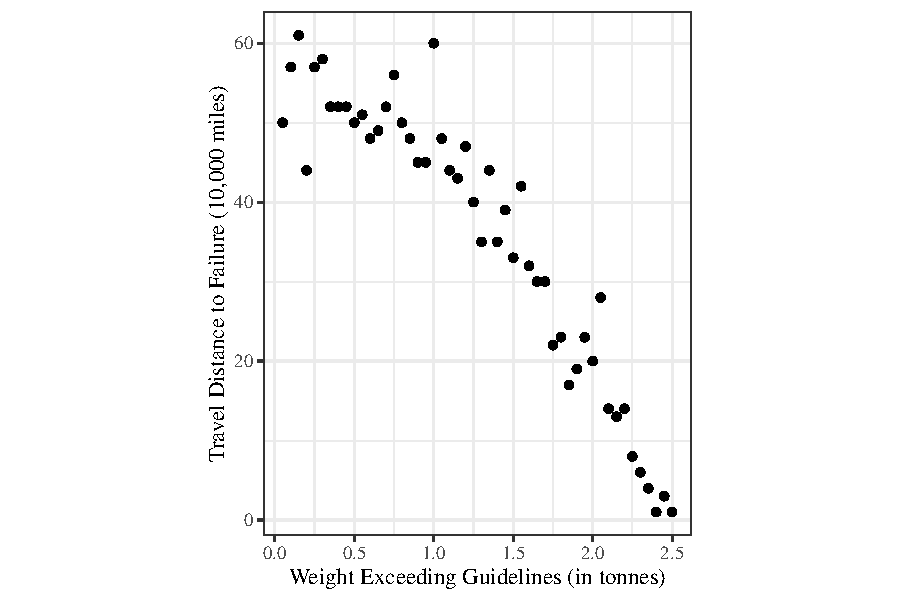
\includegraphics{stat305-hw4-003}
\end{center}

Here are some summaries of the data:

$$
\sum_{i=1}^{50} x_i = 64 \hspace{3cm} \sum_{i=1}^{50} x_i^2 = 107 \\
$$

$$
\sum_{i=1}^{50} y_i = 1795 \hspace{3cm} \sum_{i=1}^{50} y_i^2 = 79777 \\
$$

$$
\sum_{i=1}^{50} x_i y_i = 1699
$$

\begin{enumerate}
       \item  Using the summaries above, fit a linear relationship between \textbf{weight exceeding guidelines} (x) and \textbf{travel distance to failure} (y).[10 pts]
   

      \item Write the equation of the fitted linear relationship. [5 pts] 
      
      \item Find and \underline{interpret} the value of $R^2$ for the fitted linear relationship.[5 pts]
      
      \item Using the fitted line, provide a predicted value of travel distance to failure when the weight exceeding the guidelines is 3.4 tonnes.[5 pts]
      \item If the observed travel distance is $0.37$ when the weight exceeding the guidelines is 3.4, what is the residual? Based on the sign of the residual, explain if we are overfitting or under fitting.[5 pts]\\
      \emph{Hint:} You have already achieved the predicted value of travel distance when the weight exceeding the guideline is 3.4 in part (d).
      % \item Sketch what you believe the plot of residuals vs weight would look like. Why would this be a problem?[5 pts]
      % \vspace{2cm}

%
\vspace{0.3cm}
The JMP output below comes from fitting a quadratic model using $x$ and $x^2$.
\vspace{0.3cm}
    
    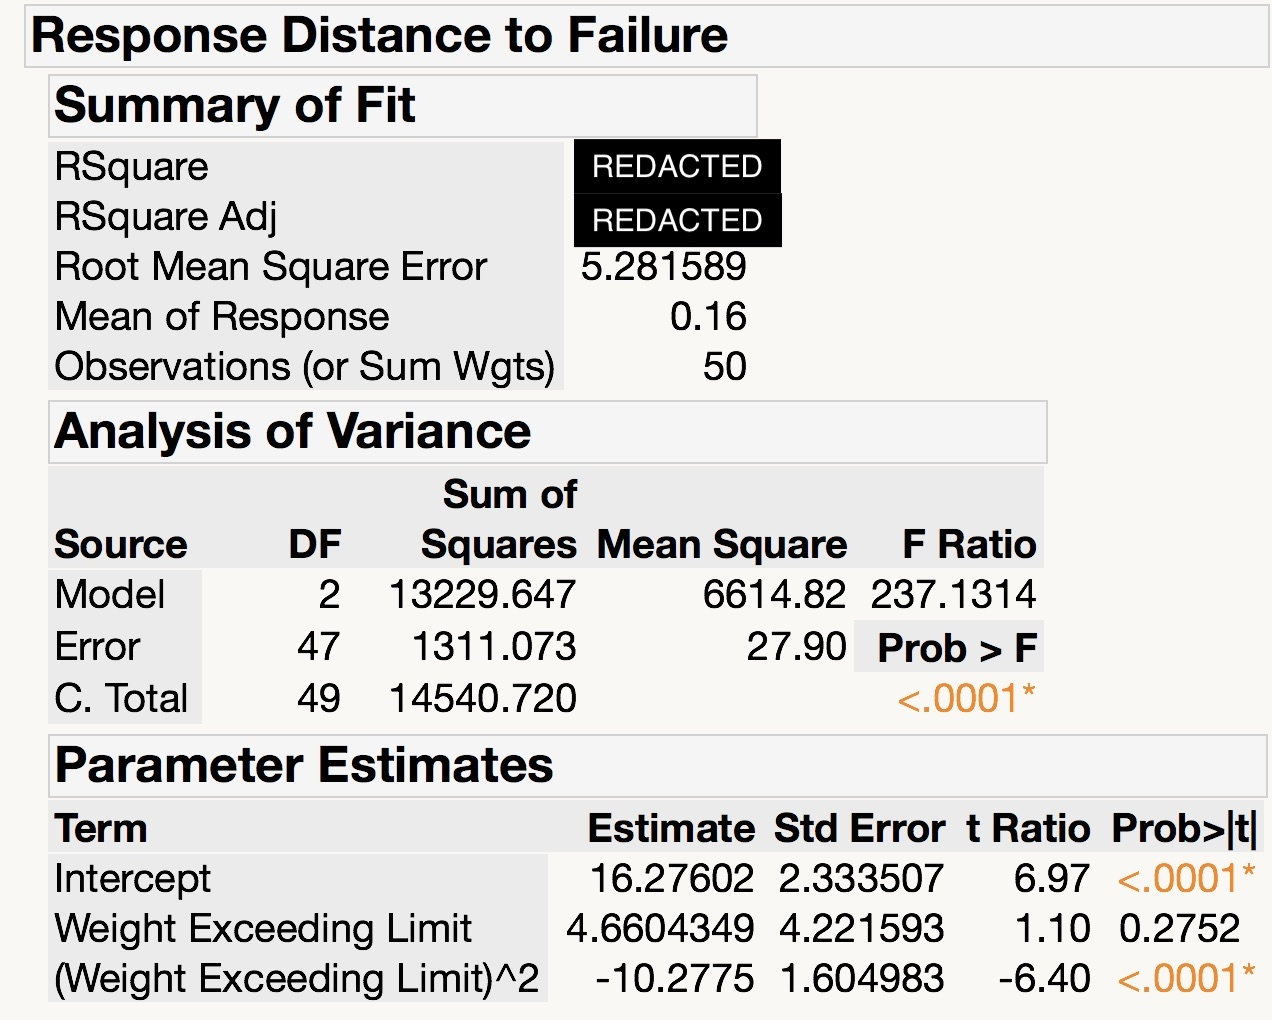
\includegraphics[scale=.2]{FitModel}

\vspace{0.3cm}
       \item Write the equation of the fitted quadratic relationship. [5 pts]
       \item Find and \underline{interpret} the value of $R^2$ for the fitted quadratic relationship.[5 pts]
       \item Using the fitted quadratic relationship, provide a predicted value of travel distance to failure when the weight exceeding the guidelines is 3.4 tonnes.[5 pts]

\end{enumerate}




	
	\item \textbf{[Ch. 4.1 Exercise 3, pg. 140]} The article "Polyglycol Modified Poly (Ethylene EtherCarbonate) Polyols by Molecular Weight Advancement" by R. Harris (*Journal of Applied Polymer Science*, 1990) contains some data on the effect of reaction temperature on the molecular weight of resulting poly polyols. The data for eight experimental runs at temperature 165°C and above are as follows (see website for `polyols.csv`):
\begin{center}
\begin{tabular}{r|r}
    \hline
    Pot temperature (°C) & Average molecular weight\\
    \hline
    165 & 808\\
    \hline
    176 & 940\\
    \hline
    188 & 1183\\
    \hline
    205 & 1545\\
    \hline
    220 & 2012\\
    \hline
    235 & 2362\\
    \hline
    250 & 2742\\
    \hline
    260 & 2935\\
    \hline
\end{tabular}
\end{center}
	
Use a statistical package (JMP or `R`) to help you complete the following (plots and computation):

   \begin{enumerate} 
    \item What fraction of the observed raw variation in molecular weight of resulting poly polyols ($y$) is accounted for by a linear equation in reaction temperature ($x$)?[5 pts]\\
    \emph{hint:} The question asks for the coefficient of determination.
    
    \item Fit a linear relationship $y \approx \beta_0 + \beta_1 x$ to these data via least squares. Then explain  how the average mulecular weight changes if pot temperature increases for a $1$°C ?[5pts]
    
    \item Compute and plot residuals from the linear relationship fit in b). Discuss what they suggest about the appropriateness of that fitted equation.[10 pts]\\
    \textbf{Note:} You should provide both residual plots vs. experimental variable and normal QQ-plot vs. residual quantiles to see if the assumptions of the model are met. 
    

    \item Based on your analysis of these data, what average molecular weight would you predict for an additional reaction run at $188$°C? At $200$°C? Why would or wouldn't you be willing to make a similar prediction of average molecular weight if the reaction is run at $70$°C?[6 pts]\\
    \emph{Hint:} You may consider extrapolation and/or intrapolation.
	
	\end{enumerate}

	
	\item  \textbf{[Ch. 4.2, Exercise 1, pg. 161]} Return to problem 2, (Exercise 3 of Section 4.1 on pg. 140 of the textbook). 
	\begin{enumerate}
	
	  \item Fit a quadratic relationship $y \approx \beta_0 + \beta_1 x + \beta_2 x^2$ to the data via least squares.[5 pts] 
	  \item Provide the value of $R^2$ and interpret that.[5 pts]
	  \item Plot residuals against the experiemntal variable and normal QQ-plot and discuss if the assumptions of the model are met.[5 pts]
	 
  \end{enumerate}



\end{enumerate}	

Total: 86 pts









\end{document}
